
\let\negmedspace\undefined
\let\negthickspace\undefined
\documentclass[journal]{IEEEtran}
\usepackage[a5paper, margin=10mm, onecolumn]{geometry}
%\usepackage{lmodern} % Ensure lmodern is loaded for pdflatex
\usepackage{tfrupee} % Include tfrupee package

\setlength{\headheight}{1cm} % Set the height of the header box
\setlength{\headsep}{0mm}     % Set the distance between the header box and the top of the text

\usepackage{gvv-book}
\usepackage{gvv}
\usepackage{cite}
\usepackage{amsmath,amssymb,amsfonts,amsthm}
\usepackage{algorithmic}
\usepackage{graphicx}
\usepackage{textcomp}
\usepackage{xcolor}
\usepackage{txfonts}
\usepackage{listings}
\usepackage{enumitem}
\usepackage{mathtools}
\usepackage{gensymb}
\usepackage{comment}
\usepackage[breaklinks=true]{hyperref}
\usepackage{tkz-euclide}
\usepackage{multicol}
\usepackage{listings}
% \usepackage{gvv}                                        
\def\inputGnumericTable{}                                 
\usepackage[latin1]{inputenc}                                
\usepackage{color}                                            
\usepackage{array}                                            
\usepackage{longtable}                                       
\usepackage{calc}                                             
\usepackage{multirow}                                         
\usepackage{hhline}
\usepackage{ifthen}                                           
\usepackage{lscape}
\usepackage{circuitikz}


\renewcommand{\thefigure}{\theenumi}
\renewcommand{\thetable}{\theenumi}
\setlength{\intextsep}{10pt} % Space between text and floats


\numberwithin{equation}{enumi}
\numberwithin{figure}{enumi}
\renewcommand{\thetable}{\theenumi}

\begin{document}
\bibliographystyle{IEEEtran}


\begin{center}
    \LARGE \textbf{GATE 2011 MA}\\[0.5em]
    \large \textbf{AI25BTECH11012 - UNNATHI GARIGE}
\end{center}

\noindent
\textbf{Q. 1 -- Q. 25 carry one mark each.}
\vspace{1em}


\begin{enumerate}


\item The distinct eigenvalues of the matrix
\begin{align*}
 \myvec{
1 & 1 & 0 \\
1 & 1 & 0 \\
0 & 0 & 0
}
\end{align*}
are
\hfill{\text{GATE MA 2011}}
\begin{multicols}{4}
\begin{enumerate}
    \item 0 and 1
    \item 1 and -1
    \item 1 and 2 
    \item 0 and 2
\end{enumerate}
\end{multicols}


% Q.2
\item The minimal polynomial of the matrix
\begin{align*}
\myvec{
3 & 3 & 0 \\
3 & 3 & 0 \\
0 & 0 & 6
}
\end{align*}
is
\hfill{\text{GATE MA 2011}}
\begin{multicols}{4}
\begin{enumerate}
    \item $x(x-1)(x-6)$
    \item $x(x-3)$
    \item $(x-3)(x-6)$
    \item  $x(x-6)$
\end{enumerate}
\end{multicols}



% Q.3
\item Which of the following is the imaginary part of a possible value of $\ln(\sqrt{i})$?
\hfill{\text{GATE MA 2011}}
\begin{multicols}{4}
\begin{enumerate}
    \item $\pi$
    \item $\frac{\pi}{2}$
    \item $\frac{\pi}{4}$ 
    \item  $\frac{\pi}{8}$
\end{enumerate}
\end{multicols}


% Q.4
\item Let $f : \mathbb{C} \to \mathbb{C}$ be analytic except for a simple pole at $z=0$ and let $g : \mathbb{C} \to \mathbb{C}$ be analytic. Then,
\begin{align*}
\frac{\text{Res}{z=0} \, f(z) g(z)}{\text{Res}{z=0} \, f(z)}
\end{align*}
is
\hfill{\text{GATE MA 2011}}
\begin{multicols}{4}
\begin{enumerate}
    \item $g(0)$
    \item $g'(0)$
    \item $\lim\limits_{z \to 0} z f(z)$
    \item $\lim\limits_{z \to 0} z f(z) g(z)$
\end{enumerate}
\end{multicols}


% Q.5
\item Let $I = \oint_C (2x^2 + y^2) \, dx + e^y \, dy$, where $C$ is the boundary (oriented anticlockwise) of the region in the first quadrant bounded by $y = 0$, $x^2 + y^2 = 1$ and $x = 0$. The value of $I$ is
\hfill{\text{GATE MA 2011}}
\begin{multicols}{4}
\begin{enumerate}
    \item $-1$
    \item $\frac{2}{3}$
    \item $\frac{2}{3}$
    \item $1$
\end{enumerate}
\end{multicols}


% Q.6
\item The series $\sum\limits_{m=1}^{\infty} \frac{\ln^m x}{m!}, \, x > 0$, is convergent on the interval
\hfill{\text{GATE MA 2011}}
\begin{multicols}{4}
\begin{enumerate}
    \item $(0, 1/e)$
    \item $(1/e, e)$ 
    \item $(0, e)$
    \item $(1, e)$
\end{enumerate}
\end{multicols}


% Q.7
\item While solving the equation $x^2 - 3x + 1 = 0$ using the Newton--Raphson method with the initial guess of a root as $1$, the value of the root after one iteration is
\hfill{\text{GATE MA 2011}}
\begin{multicols}{4}
\begin{enumerate}
    \item $1.5$ 
    \item $1$
    \item  $0.5$
    \item $0$
\end{enumerate}
\end{multicols}






% Q.8
\item Consider the system of equations
\begin{align*}
\myvec{
5 & 2 & 1 \\
-2 & 5 & 2 \\
-1 & 2 & 8
}
\myvec{
x_1 \\ x_2 \\ x_3
}
=
\myvec{
13 \\ -22 \\ 14
}
\end{align*}
With the initial guess of the solution $(x_1, x_2, x_3)^T = (1, 1, 1)^T$, the approximate value of the solution $(x_1, x_2, x_3)^T$ after one iteration by the Gauss Seidel method is

\hfill{\text{GATE MA 2011}}
\begin{multicols}{2}
\begin{enumerate}
    \item $[2, -4.4, 1.625]^T$
    \item $[2, -4, -3]^T$
    \item  $[2, 4.4, 1.625]^T$ 
    \item $[2, -4, 3]^T$

\end{enumerate}
\end{multicols}



% Q.9
\item Let $y$ be the solution of the initial value problem
\begin{align*}
\frac{dy}{dx} = y^2 + x, \quad y(0) = 1.
\end{align*}
Using Taylor series method of order 2 with the step size $h = 0.1$, the approximate value of $y(0.1)$ is
\hfill{\text{GATE MA 2011}}
\begin{multicols}{4}
\begin{enumerate}
    \item $1.315$ 
    \item $1.415$
    \item $1.115$
    \item $1.215$

\end{enumerate}
\end{multicols}


% Q.10
\item The partial differential equation
\begin{align*}
x^2 \frac{\partial^2 z}{\partial x^2} + (y^2 - 1) \frac{\partial^2 z}{\partial x \partial y} + (y^2 - 1) \frac{\partial^2 z}{\partial y^2} + \frac{\partial z}{\partial x} + y \frac{\partial z}{\partial y} = 0
\end{align*}
is hyperbolic in a region in the $XY$ plane if
\hfill{\text{GATE MA 2011}}
\begin{multicols}{4}
\begin{enumerate}
    \item $x \neq 0$ and $y = 1$ 
    \item $x \neq 0$ and $y \neq 1$
    \item $x = 0$ and $y \neq 1$
    \item $x = 0$ and $y = 1$
\end{enumerate}
\end{multicols}



% Q.11
\item Which of the following functions is a probability density function of a random variable $X$?
\hfill{\text{GATE MA 2011}}
\begin{multicols}{2}
\begin{enumerate}
    \item $f(x) = \begin{cases} x(2-x), & 0 < x < 2 \\ 0, & \text{elsewhere} \end{cases}$
    \item $f(x) = \begin{cases} x(1-x), & 0 < x < 1 \\ 0, & \text{elsewhere} \end{cases}$
    \item $f(x) = \begin{cases} 2x e^{-x^2}, & -1 < x < 1 \\ 0, & \text{elsewhere} \end{cases}$
    \item $f(x) = \begin{cases} 2x e^{-x}, & x > 0 \\ 0, & \text{elsewhere} \end{cases}$
\end{enumerate}
\end{multicols}


% Q.12
\item Let $X_1, X_2, X_3, X_4$ be independent standard normal random variables.  
The distribution of
\begin{align*}
W = \frac{1}{2} \left( (X_1 - X_2)^2 + (X_3 - X_4)^2 \right)
\end{align*}
is
\hfill{\text{GATE MA 2011}}
\begin{multicols}{4}
\begin{enumerate}
    \item $N(0, 1)$
    \item $N(0, 2)$
    \item $\chi^2_2$
    \item $\chi^2_4$
\end{enumerate}
\end{multicols}




% Q.13
\item For $n \ge 1$, let $\{X_n\}$ be a sequence of independent random variables with
\begin{align*}
P(X_n = n) = P(X_n = -n) = \frac12
\end{align*}

Then, which of the following statements is \textbf{TRUE} for the sequence $\{X_n\}$?
\hfill{\text{GATE MA 2011}}

\begin{enumerate}
\item  Weak Law of Large Numbers holds but Strong Law of Large Numbers does not hold 
\item  Weak Law of Large Numbers does not hold but Strong Law of Large Numbers holds 
\item  Both Weak Law of Large Numbers and Strong Law of Large Numbers hold 
\item  Both Weak Law of Large Numbers and Strong Law of Large Numbers do not hold
 \end{enumerate}

% Q14
\item  The Linear Programming Problem: \\
Maximize $z = x_1 + x_2$ 
subject to
\begin{align*}
x_1 + 2x_2 &\le 20, \\
x_1 + x_2 &\le 15, \\
x_2 &\le 6, \\
x_1, x_2 &\ge 0
\end{align*}
\hfill{\text{GATE MA 2011}}
\begin{multicols}{2}
\begin{enumerate}
\item  has exactly one optimum solution 
\item  has more than one optimum solutions  
\item  has unbounded solution 
\item  has no solution
\end{enumerate}
\end{multicols}


% Q15
\item  Consider the Primal Linear Programming Problem: \\
Maximize  $z = c_1x_1 + c_2x_2 + \dots + c_nx_n$  \\
subject to \hfill{\text{GATE MA 2011}}

\begin{align*}
\text{P:} \quad
\begin{cases}
a_{11}x_1 + a_{12}x_2 + \dots + a_{1n}x_n \le b_1, \\
a_{21}x_1 + a_{22}x_2 + \dots + a_{2n}x_n \le b_2, \\
\quad \vdots \\
a_{m1}x_1 + a_{m2}x_2 + \dots + a_{mn}x_n \le b_m, \\
x_j \ge 0, \quad j=1,\dots,n
\end{cases}
\end{align*}
The Dual of P is \\
Minimize \quad $z' = b_1w_1 + b_2w_2 + \dots + b_mw_m$ \\
subject to
\begin{align*}
\text{D:} \quad
\begin{cases}
a_{11}w_1 + a_{21}w_2 + \dots + a_{m1}w_m \ge c_1, \\
a_{12}w_1 + a_{22}w_2 + \dots + a_{m2}w_m \ge c_2, \\
\quad \vdots \\
a_{1n}w_1 + a_{2n}w_2 + \dots + a_{mn}w_m \ge c_n, \\
w_i \ge 0, \quad i=1,\dots,m
\end{cases}
\end{align*}
Which of the following statements is \textbf{FALSE}?
\begin{enumerate}
\item  If P has an optimal solution, then D also has an optimal solution 
\item  The dual of the dual problem is a primal problem 
\item  If P has an unbounded solution, then D has no feasible solution 
\item  If P has no feasible solution, then D has a feasible solution
\end{enumerate}


% Q16
\item The number of irreducible quadratic polynomials over the field of two elements $F_2$ is
\hfill{\text{GATE MA 2011}}
\begin{multicols}{4}
\begin{enumerate}
    \item 0
    \item 1
    \item 2
    \item 3
\end{enumerate}
\end{multicols}



% Q17
\item The number of elements in the conjugacy class of the $3$-cycle $(2\ 3\ 4)$ in the symmetric group $S_6$ is
\hfill{\text{GATE MA 2011}}
\begin{multicols}{4}
\begin{enumerate}
    \item 20
    \item 40
    \item 120
    \item 216
\end{enumerate}
\end{multicols}


\item The initial value problem  
\begin{align*}
x \frac{dy}{dx} = y + x^2, \quad x > 0; \quad y(0) = 0,
\end{align*}
has 
\hfill{\text{GATE MA 2011}}
\begin{multicols}{2}
\begin{enumerate}
    \item infinitely many solutions
    \item exactly two solutions
    \item a unique solution
    \item no solution
\end{enumerate}
\end{multicols}




\item The subspace $P = \{(x,y,z)\in \mathbb{R}^3 : z = x^2 + y^2 + 1\}$ is
\hfill{\text{GATE MA 2011}}
\begin{multicols}{2}
\begin{enumerate}
    \item compact and connected
    \item compact but not connected
    \item not compact but connected 
    \item neither compact nor connected

\end{enumerate}
\end{multicols}


\item Let

$P = (0,1); Q = [0,1]; U = (0,1]; S = [0,1]; T = \mathbb{R}$ and $A = \{P,Q,U,S,T\}$

The equivalence relation 'homeomorphism' induces which one of the following as the partition of $A$?
\hfill{\text{GATE MA 2011}}
\begin{multicols}{2}
\begin{enumerate}
    \item $\{P,Q,U,S\}, \{T\}$
    \item $\{P,T\}, \{Q\}, \{U\}, \{S\}$
    \item $\{P,T\}, \{Q,U,S\}$ 
    \item $\{P,T\}, \{Q,U\}, \{S\}$
\end{enumerate}
\end{multicols}



\item Let $x = (x_1, x_2, \dots) \in l^p, x \neq 0$. For which one of the following values of $p$, the series $\sum_{i=1}^{\infty} x_i y_i$ converges for every $y = (y_1, y_2, \dots) \in l^{p'}$?
\hfill{\text{GATE MA 2011}}
\begin{multicols}{4}
\begin{enumerate}
    \item 1
    \item 2
    \item 3
    \item 4
\end{enumerate}
\end{multicols}



\item Let $H$ be a complex Hilbert space and $H'$ be its dual. The mapping $\phi : H \to H'$ defined by $\phi(y) = f_{y}$ where $f_{y}(x) = \langle x, y \rangle$ is
\hfill{\text{GATE MA 2011}}
\begin{multicols}{2}
\begin{enumerate}
    \item not linear but onto
    \item both linear and onto
    \item linear but not onto
    \item neither linear nor onto
\end{enumerate}
\end{multicols}




\item A horizontal lever is in static equilibrium under the application of vertical forces $F_1$ at a distance $l_1$ from the fulcrum and $F_2$ at a distance $l_2$ from the fulcrum. The equilibrium for the above quantities can be obtained if
\hfill{\text{GATE MA 2011}}
\begin{multicols}{4}
\begin{enumerate}
    \item $F_1 l_1 = 2F_2 l_2$
    \item $2F_1l_1 = F_2 l_2$
    \item $F_1l_1 = F_2 l_2$
    \item $F_1l_1 < F_2 l_2$
\end{enumerate}
\end{multicols}



\item Assume $F$ to be a twice continuously differentiable function.\\
Let $J(y)$ be a functional of the form  \hfill{\text{GATE MA 2011}}
\begin{align*}
J(y) = \int_0^1 F(x, y') dx, \quad 0 \leq x \leq 1
\end{align*}
defined on the set of all continuously differentiable functions $y$ on $[0,1]$ satisfying $y(0) = a$, $y(1) = b$. For some arbitrary constant $c$, a necessary condition for $y$ to be an extremum of $J$ is
\begin{multicols}{4}
\begin{enumerate}
    \item $\frac{\partial F}{\partial x} = c$ \hspace{1cm}
    \item $\frac{\partial F}{\partial y'} = c$ \hspace{1cm}
    \item $\frac{\partial F}{\partial y} = c$ \hspace{1cm}
    \item $\frac{\partial F}{\partial x} = 0$
\end{enumerate}
\end{multicols}


\item The eigenvalue $\lambda$ of the following Fredholm integral equation
\begin{align*}
y(x) = \lambda \int_{0}^{1} x^{2} t \, y(t) \, dt
\end{align*}
is
\hfill{\text{GATE MA 2011}}
\begin{multicols}{4}
\begin{enumerate}
    \item -2
    \item 2
    \item 4
    \item -4
\end{enumerate}
\end{multicols}



\item The application of Gram Schmidt process of orthonormalization to 
\begin{align*}
u_1 = (1,1,0), \quad u_2 = (1,0,0), \quad u_3 = (1,1,1)
\end{align*}
yields
\hfill{\text{GATE MA 2011}}
\begin{multicols}{2}
\begin{enumerate}
    \item $\frac{1}{\sqrt{2}}(1,1,0),\ (1,0,0),\ (0,0,1)$
    \item $\frac{1}{\sqrt{2}}(1,1,0),\ \frac{1}{\sqrt{2}}(1,-1,0),\ \frac{1}{\sqrt{2}}(1,1,1)$
    \item  $\frac{1}{\sqrt{2}}(1,1,0),\ \frac{1}{\sqrt{2}}(1,-1,0),\ (0,0,1)$
    \item  $(0,1,0),\ (1,0,0),\ (0,0,1)$
\end{enumerate}
\end{multicols}



\item Let $T:\mathbb{C}^3 \to \mathbb{C}^3$ be defined by 
\begin{align*}
T \myvec{z_1 \\ z_2 \\ z_3 } =
\myvec{
z_1 + i z_2 \\
i z_1 + z_2 \\
z_1 + z_2 + i z_3}
.\end{align*}

Then, the adjoint $T^*$ of $T$ is given by 
\hfill{\text{GATE MA 2011}}
\begin{align*}
  T \myvec{ z_1 \\ z_2 \\ z_3 }  
\end{align*}
\begin{multicols}{4}
\begin{enumerate}
\item  $\myvec{ z_1 + i z_2 \\ -i z_1 + z_2 \\ z_1 + z_2 - i z_3}$
\item  $\myvec{ z_1 - i z_2 + z_3 \\ i z_1 + z_2 + z_3 \\ i z_3 }$
\item  $\myvec{ z_1 - i z_2 + z_3 \\ i z_1 + z_2 + z_3 \\ -i z_3 }$
\item  $\myvec{ i z_1 + z_2 \\ z_1 - i z_2 \\ z_1 - i z_2 - i z_3}$
\end{enumerate}
\end{multicols}

\item Let $f(z)$ be an entire function such that $\ |f(z)| \leq K\,|z|,\ \forall z \in \mathbb{C}$, for some $K>0$.
If $f(i) = i$, the value of $f'(i)$ is
\hfill{\text{GATE MA 2011}}
\begin{multicols}{4}
\begin{enumerate}
\item  $1$ \hspace{2cm}
\item  $-1$ \hspace{2cm}
\item  $i$ \hspace{2cm}
\item  $-i$
\end{enumerate}
\end{multicols}

\item Let $y$ be the solution of the initial value problem
\hfill{\text{GATE MA 2011}}
\begin{align*}
\frac{d^2 y}{d x^2} + y = 6 \cos 2x,\quad y(0) = 3,\quad y'(0) = 1.
\end{align*}
Let the Laplace transform of $y$ be $F(s)$. Then, the value of $F(1)$ is\\
\begin{multicols}{4}
\begin{enumerate}
\item  $\frac{17}{5}$ \hspace{2cm}
\item  $\frac{13}{5}$ \hspace{2cm}
\item  $\frac{11}{5}$ \hspace{2cm}
\item  $\frac{9}{5}$
\end{enumerate}
\end{multicols}


\item For $0 \leq x \leq 1$, let   \hfill{\text{GATE MA 2011}}

\begin{align*}
f_n(x) =
\begin{cases}
\frac{n}{1+n}, & \text{if $x$ is irrational}, \\
0, & \text{if $x$ is rational}.
\end{cases}
\end{align*}
and $f(x) = \lim\limits_{n \to \infty} f_n(x)$.
Then, on the interval $[0,1]$,\\
\begin{enumerate}
    \item $f$ is measurable and Riemann integrable
    \item $f$ is measurable and Lebesgue integrable
    \item $f$ is not measurable
    \item $f$ is not Lebesgue integrable
\end{enumerate}




\item If $x$, $y$, and $z$ are positive real numbers, then the minimum value of \hfill{\text{GATE MA 2011}}
\begin{align*}
 x^2 + 8y^2 + 27z^2
\end{align*}
\begin{multicols}{4}
\begin{enumerate}
    \item  108 \hspace{2cm}
    \item  216 \hspace{2cm}
    \item  405 \hspace{2cm}
    \item  1048
\end{enumerate}
\end{multicols}
  

\item Let $T:\mathbb{R}^4 \to \mathbb{R}^4$ be defined by
\begin{align*}
 T(x, y, z, w) = (x + y + 5w, x + 2y + w, -z + 2w, 5x + y + 2z).   
\end{align*}

The dimension of the eigenspace of $T$ is  
\hfill{\text{GATE MA 2011}}
\begin{multicols}{4}
\begin{enumerate}
\item  $1$ \hspace{2cm}
\item  $2$ \hspace{2cm}
\item  $3$ \hspace{2cm}
\item  $4$
\end{enumerate}
\end{multicols}




\item Let $y$ be a polynomial solution of the differential equation
\begin{align*}
(1 - x^2)y'' - 2xy' + 6y = 0.
\end{align*}
If $y(1) = 2$, then the value of the integral $\displaystyle\int_{-1}^{1} y^2 \, dx$ is
\hfill{\text{GATE MA 2011}}
\begin{multicols}{4}
\begin{enumerate}
\item $\frac{1}{5}$ \hspace{2cm}
\item  $\frac{2}{5}$ \hspace{2cm}
\item  $\frac{4}{5}$ \hspace{2cm}
\item  $\frac{8}{5}$ 
\end{enumerate}
\end{multicols}


    

\item The value of the integral
\begin{align*}
I = \int_1^2 \exp(x^2) dx
\end{align*}
using a rectangular rule is approximated as $2$. Then, the approximation error $|I - 2|$ lies in the interval
\hfill{\text{GATE MA 2011}}
\begin{multicols}{4}
\begin{enumerate}
\item  $(2e, 3e]$ \hspace{2cm}
\item  $(2/3, 2e]$ \hspace{2cm}
\item  $(e/8, 2/3]$ \hspace{2cm}
\item  $(0, e/8]$
\end{enumerate}
\end{multicols}

    
\item The integral surface for the Cauchy problem
\begin{align*}
\frac{\partial z}{\partial x} + \frac{\partial z}{\partial y} = 1,
\end{align*}
which passes through the circle $z = 0$, $x^2 + y^2 = 1$ is
\hfill{\text{GATE MA 2011}}
\begin{enumerate}
    \item $x^2 + y^2 + 2z^2 + 2zx - 2yz - 1 = 0$
    \item $x^2 + y^2 + 2z^2 + 2zx + 2yz - 1 = 0$
    \item $x^2 + y^2 + 2z^2 - 2zx - 2yz - 1 = 0$
    \item $x^2 + y^2 + 2z^2 + 2z + 2yz + 1 = 0$
\end{enumerate}


 
\item \text{The vertical displacement } u(x, t) \text{ of an infinitely long elastic string is governed by the initial value problem}
\begin{align*}
\frac{\partial^2 u}{\partial t^2} = 4 \frac{\partial^2 u}{\partial x^2}, \quad -\infty < x < \infty, \; t > 0,
\end{align*}
\begin{align*}
u(x, 0) = -x \quad \text{and} \quad \frac{\partial u}{\partial t}(x, 0) = 0.
\end{align*}
\text{The value of } u(x, t) \text{ at } x=2 \text{ and } t=2 \text{ is equal to}
\hfill{\text{GATE MA 2011}}
\begin{multicols}{4}
\begin{enumerate}
\item  2
\item  4 
\item  -2 
\item  -4
\end{enumerate}
\end{multicols}






\item We have to assign four jobs I, II, III, IV to four workers $A, B, C,$ and $D$. The time taken by different workers (in hours) in completing different jobs is given below:

\begin{align*}
\begin{array}{|c|c|c|c|c|}
   \hline
    & \text{I} & \text{II} & \text{III} & \text{IV} \\
    \hline
    A & 5 & 3 & 2 & 8 \\
    B & 7 & 9 & 2 & 6 \\
    C & 8 & 5 & 1 & 7 \\
    D & 5 & 7 & 7 & 8 \\
    \hline
\end{array}
\end{align*}

The optimal assignment is as follows: \\
Job III to worker A; Job IV to worker B; Job II to worker C; Job I to worker D and hence the time taken by different workers in completing different jobs is now changed as:

\begin{align*}
\begin{array}{|c|c|c|c|c|}
 \hline
    & \text{I} & \text{II} & \text{III} & \text{IV} \\
    \hline
    A & 7 & 9 & 2 & 5 \\
    B & 8 & 7 & 9 & 2 \\
    C & 4 & 2 & 7 & 5 \\
    D & 5 & 7 & 7 & 5 \\
     \hline
\end{array}
\end{align*}

Then the minimum time (in hours) taken by the workers to complete all the jobs is
\hfill{\text{GATE MA 2011}}
\begin{multicols}{4}
\begin{enumerate}
\item  10 
\item  12 
\item  15 
\item  17
\end{enumerate}
\end{multicols}



\item The following table shows the information on the availability of supply to each warehouse, the requirement of each market and unit transportation cost (in rupees) from each warehouse to each market. 

\begin{align*}
\begin{array}{|c|c|c|c|c|c|}
   \hline
    & M_1 & M_2 & M_3 & M_4 & \text{Supply} \\
    \hline
    W_1 & 6 & 3 & 5 & 4 & 22 \\
    W_2 & 5 & 9 & 8 & 7 & 15 \\
    W_3 & 7 & 5 & 9 & 8 & 8 \\
    \hline
    \text{Requirement} & 7 & 12 & 17 & 9 & \\
    \hline
\end{array}
\end{align*}

The present transportation schedule is as follows: \\
$W_1$ to $M_2$: 12 units; $W_1$ to $M_1$: 1 unit; $W_1$ to $M_4$: 9 units; $W_2$ to $M_3$: 15 units; $W_3$ to $M_1$: 7 units and $W_3$ to $M_3$: 1 unit. Then the minimum total transportation cost (in rupees) is
\hfill{\text{GATE MA 2011}}
\begin{multicols}{4}
\begin{enumerate}
\item  150
\item  149
\item  148 
\item  147 
\end{enumerate}
\end{multicols}


\item If $\mathbb{Z}[i]$ is the ring of Gaussian integers, the quotient $\mathbb{Z}[i]/(3-i)$ is isomorphic to
\hfill{\text{GATE MA 2011}}
\begin{multicols}{4}
\begin{enumerate}
\item  Z
\item  Z/$3$Z
\item  Z/$4$Z
\item  Z/$10$Z 
\end{enumerate}
\end{multicols}




\item For the rings
\begin{align*}
L = \frac{\mathbb{R}[x]}{(x^2 - x + 1)}, \quad
M = \frac{\mathbb{R}[x]}{(x^2 + x + 1)}, \quad
N = \frac{\mathbb{R}[x]}{(x^2 + 2x + 1)}
\end{align*}
which one of the following is \textbf{TRUE}?
\hfill{\text{GATE MA 2011}}
\begin{enumerate}
    \item $L$ is isomorphic to $M$; $L$ is not isomorphic to $N$; $M$ is not isomorphic to $N$
    \item  $M$ is isomorphic to $N$; $M$ is not isomorphic to $L$; $N$ is not isomorphic to $L$
    \item $L$ is isomorphic to $M$; $M$ is isomorphic to $N$
    \item $L$ is not isomorphic to $M$; $L$ is not isomorphic to
    \end{enumerate}
    

\item The time to failure (in hours) of a component is a continuous random variable $T$ with the probability density function
    \begin{align*}
        f(t) = 
        \begin{cases}
            \frac{1}{10} e^{-t/10}, & t > 0, \\
            0, & t \leq 0
        \end{cases}
     \end{align*}
    Ten of these components are installed in a system and they work independently. Then, the probability that NONE of these fail before ten hours, is
\hfill{\text{GATE MA 2011}}
\begin{multicols}{4}
\begin{enumerate}
\item  $e^{-10}$
\item  $1 - e^{-10}$
\item  $10 e^{-10}$
\item  $1 - 10 e^{-10}$
\end{enumerate}
\end{multicols}

     
    
    \item Let $X$ be the real normed linear space of all real sequences with finitely many non-zero terms, with supremum norm and $T : X \to X$ be a one to one and onto linear operator defined by
    \begin{align*}
        T(x_1, x_2, x_3, \ldots) = (x_1, \frac{x_2}{2}, \frac{x_3}{3}, \ldots).
     \end{align*}
    Then, which of the following is \textbf{TRUE}?
    \hfill{\text{GATE MA 2011}}
\begin{multicols}{2}
\begin{enumerate}
\item  $T$ is bounded but $T^{-1}$ is not bounded
\item  $T$ is not bounded but $T^{-1}$ is bounded
\item  Both $T$ and $T^{-1}$ are bounded
\item  Neither $T$ nor $T^{-1}$ is bounded
\end{enumerate}
\end{multicols}

    
    
    \item Let $e_i = (0, \ldots, 0, 1, 0, \ldots)$ (i.e., $e_i$ is the vector with $1$ at the $i^\text{th}$ place and $0$ elsewhere) for $i = 1, 2, \ldots$. \\
    Consider the statements: \\
    P: $\{f(e_i)\}$ converges for every continuous linear functional on $l^2$. \\
    Q: $\{e_i\}$ converges in $l^2$. \\
    Then, which of the following holds?
\hfill{\text{GATE MA 2011}}
\begin{multicols}{2}
\begin{enumerate}
\item  Both P and Q are TRUE
\item  P is TRUE but Q is not TRUE
\item  P is not TRUE but Q is TRUE
\item  Neither P nor Q is TRUE
\end{enumerate}
\end{multicols}
    

    
\item For which subspace $X \subseteq \mathbb{R}$ with the usual topology and with $\{0,1\} \subseteq X$, will a continuous function $f : X \to \{0, 1\}$ satisfying $f(0) = 0$ and $f(1) = 1$ exist?
 \hfill{\text{GATE MA 2011}}
\begin{multicols}{2}
\begin{enumerate}
\item  $X = [0,1]$
\item $X = [-1,1]$
\item $X = \mathbb{R}$
\item $[0,1] \subset X$
\end{enumerate}
\end{multicols}



 \item Suppose $X$ is a finite set with more than five elements. Which of the following is\\ \textbf{TRUE}?   \hfill{\text{GATE MA 2011}}

\begin{enumerate}
    \item There is a topology on $X$ which is $T_3$
    \item There is a topology on $X$ which is $T_2$ but not $T_3$
    \item There is a topology on $X$ which is $T_1$ but not $T_2$
    \item There is no topology on $X$ which is $T_1$
\end{enumerate}

 

\item A massless wire is bent in the form of a parabola \( z = r^2 \) and a bead slides on it smoothly. The wire is rotated about z-axis with a constant angular acceleration \(\alpha\). Assume that \( m \) is the mass of the bead, \(\omega\) is the initial angular velocity and \( g \) is the acceleration due to gravity. Then, the Lagrangian at any time \( t \) is
   \hfill{\text{GATE MA 2011}}

\begin{enumerate}
    \item $\frac{m}{2} \left( \frac{dr}{dt} \right)^2 \left[ (1+4r^2) + r^2 (\omega + \alpha t)^2 + 2g r^2 \right]$
    \item $\frac{m}{2} \left( \frac{dr}{dt} \right)^2 \left[ (1+4r^2) - r^2 (\omega + \alpha t)^2 + 2g r^2 \right]$
    \item $\frac{m}{2} \left( \frac{dr}{dt} \right)^2 \left[ (1+4r^2) - r^2 (\omega + \alpha t)^2 - 2g r^2 \right]$
    \item $\frac{m}{2} \left( \frac{dr}{dt} \right)^2 \left[ (1+4r^2) + r^2 (\omega + \alpha t)^2 - 2g r^2 \right]$
\end{enumerate}



\item On the interval \([0,1]\), let \( y \) be a twice continuously differentiable function which is an extremal of the functional
\begin{align*}
J(y) = \int_0^1 \frac{\sqrt{1 + 2y'^2}}{x} \, dx
\end{align*}
with \( y(0) = 1, \, y(1) = 2 \). Then, for some arbitrary constant \( c \), \( y \) satisfies
 \hfill{\text{GATE MA 2011}}
\begin{multicols}{2}
\begin{enumerate}
\item  $y'^2 (2 - c^2 x^2 ) = c^2 x^2$
\item $y'^2 (2 + c^2 x^2 ) = c^2 x^2$
\item $y'^2 (1 - c^2 x^2 ) = c^2 x^2$
\item $y'^2 (1 + c^2 x^2 ) = c^2 x^2$
\end{enumerate}
\end{multicols}

\bigskip

\textbf{Common Data Questions}
\newline
\textbf{Common Data for Questions 48 and 49:}

Let $X$ and $Y$ be two continuous random variables with the joint probability density function
\begin{align*}
f(x, y) = 
\begin{cases}
2, & 0 < x + y < 1,\, x > 0,\, y > 0, \\
0, & \text{elsewhere}.
\end{cases}
\end{align*}


\item $P\left( X + Y < \frac{1}{2} \right)$ is
\hfill{\text{GATE MA 2011}}
\begin{multicols}{4}
\begin{enumerate}
\item $\frac{1}{4}$
\item $\frac{1}{2}$
\item $\frac{3}{4}$
\item $1$
\end{enumerate}
\end{multicols}
   

\item $E\left( X \mid Y = \frac{1}{2} \right)$ is
    \hfill{\text{GATE MA 2011}}
\begin{multicols}{4}
\begin{enumerate}
\item $\frac{1}{4}$
\item $\frac{1}{2}$
\item 1
\item 2
\end{enumerate}
\end{multicols}

    


\textbf{Common Data for Questions 50 and 51:}\\
Let
\begin{align*}
f(z) = \frac{z}{8 - z^3}, \qquad z = x + iy.
\end{align*}
  
  
  \item \begin{align*}
         \operatorname{Res}_{z=2} f(z)
         \end{align*}
         is
\hfill{\text{GATE MA 2011}}
\begin{multicols}{4}
\begin{enumerate}
   \item $-\frac{1}{8}$
   \item $\frac{1}{8}$
   \item $-\frac{1}{6}$
    \item  $\frac{1}{6}$
\end{enumerate}
\end{multicols}
  

\item The Cauchy principal value of $\displaystyle \int_{-\infty}^{\infty} f(x)dx$ is
    \hfill{\text{GATE MA 2011}}
\begin{multicols}{4}
\begin{enumerate}
   \item $-\frac{\pi}{6}\sqrt{3}$
   \item $-\frac{\pi}{8}\sqrt{3}$
   \item $\pi\sqrt{3}$
    \item $-\pi\sqrt{3}$
\end{enumerate}
\end{multicols}
   

\vspace{0.5em}
\textbf{Linked Answer Questions}
\vspace{0.5em}

\textbf{Statement for Linked Answer Questions 52 and 53:}

Let 
\begin{align*}
f_n(x) = \frac{x}{\{(n-1)x + 1\}\{nx + 1\}}
\end{align*}
and
\begin{align*}
s_n(x) = \sum_{j=1}^n f_j(x) \quad \text{for } x \in [0,1].
\end{align*}

\item The sequence $\{s_n\}$
\hfill{\text{GATE MA 2011}}
 \begin{enumerate}
 \item  converges uniformly on $[0,1]$ 
 \item  converges pointwise on $[0,1]$ but not uniformly 
 \item  converges pointwise for $x = 0$ but not for $x \in (0,1]$ 
 \item  does not converge for $x \in [0,1]$
  \end{enumerate}



\item
\begin{align*}
\lim_{n \to \infty} \int_0^1 s_n(x) dx = 1
\end{align*}
\begin{enumerate}
\item by dominated convergence theorem 
\item by Fatous lemma 
\item by the fact that $\{s_n\}$ converges uniformly on $[0,1]$ 
\item by the fact that $\{s_n\}$ converges pointwise on $[0,1]$  \hfill{\text{GATE MA 2011}}
 \end{enumerate}

\vspace{0.5em}
\textbf{Statement for Linked Answer Questions 54 and 55:}\\
\vspace{0.5em}
The matrix 
\begin{align*}
A = \myvec{
1 & 1 & 1 \\
2 & 1 & 2 \\
1 & 3 & 2
}
\end{align*}
can be decomposed into the product of a lower triangular matrix $L$ and an upper triangular matrix $U$ as $A = LU$ where
\begin{align*}
L = \myvec{
1 & 0 & 0 \\
l_{21} & 1 & 0 \\
l_{31} & l_{32} & 1
}
\quad \text{and} \quad
U = \myvec{
u_{11} & u_{12} & u_{13} \\
0 & u_{22} & u_{23} \\
0 & 0 & u_{33}
}
\end{align*}

Let $x, z \in \mathbb{R}^3$ and $b = [1, 1, 1]^T$.

\item The solution $z = [z_1, z_2, z_3]^T$ of the system $Lz = b$ is
\hfill{\text{GATE MA 2011}}
\begin{multicols}{4}
\begin{enumerate}
   \item $[-1, -1, -2]^T$
   \item $[1, -1, 2]^T$
   \item $[1, -1, -2]^T$
    \item $[-1, 1, 2]^T$
\end{enumerate}
\end{multicols}




\item The solution $x = [x_1, x_2, x_3]^T$ of the system $Ux = z$ is
\hfill{\text{GATE MA 2011}}
\begin{multicols}{4}
\begin{enumerate}
   \item $[2, 1, -2]^T$
   \item $[2, 1, 2]^T$
   \item $[-2, -1, -2]^T$
    \item $[-2, 1, -2]^T$
\end{enumerate}
\end{multicols}


\vspace{1em}
\textbf{General Aptitude (GA) Questions}
\newline
\textbf{Q.56 -- Q.60 carry one mark each.}\\


\item Choose the most appropriate word from the options given below to complete the following sentence:\\
\textbf{It was her view that the country's problems had been \underline{\hspace{2cm}} by foreign technocrats, so that to invite them to come back would be counter-productive.}
\hfill{\text{GATE MA 2011}}
\begin{enumerate}
    \item identified
     \item ascertained
     \item exacerbated
     \item analysed
\end{enumerate}
    

\item There are two candidates P and Q in an election. During the campaign, 40\% of the voters promised to vote for P, and rest for Q. However, on the day of election 15\% of the voters went back on their promise to vote for P and instead voted for Q. 25\% of the voters went back on their promise to vote for Q and instead voted for P. \\ Suppose, P lost by 2 votes, then what was the total number of voters?
\hfill{\text{GATE MA 2011}}
\begin{multicols}{4}
\begin{enumerate}
   \item $100$
   \item $110$
   \item $90$
    \item $95$
\end{enumerate}
\end{multicols}


   
\item The question below consists of a pair of related words followed by four pairs of words. Select the pair that best expresses the relation in the original pair:\\
\textbf{Gladiator : Arena}

\hfill{\text{GATE MA 2011}}
\begin{enumerate}
    \item  dancer : stage
     \item commuter : train
     \item teacher : classroom
     \item lawyer : courtroom
\end{enumerate}


   
\item Choose the most appropriate word from the options given below to complete the following sentence:\\
\textbf{Under ethical guidelines recently adopted by the Indian Medical Association, human genes are to be manipulated only to correct diseases for which \underline{\hspace{2cm}} treatments are unsatisfactory.}

\begin{enumerate}
    \item   similar \hfill{\text{GATE MA 2011}}
     \item most
     \item uncommon
     \item available
\end{enumerate}

   
\item Choose the word from the options given below that is most nearly opposite in meaning to the given word:\\
\textbf{Frequency}  \hfill{\text{GATE MA 2011}}
\begin{enumerate}
    \item  periodicity 
     \item rarity
     \item gradualness
     \item persistency
\end{enumerate}

     

\textbf{Q.61 to Q.65 carry two marks each.}
\item Three friends, R, S and T shared toffee from a bowl. R took $\frac{1}{3}$ of the toffees, but returned four to the bowl. S took $\frac{1}{4}$ of what was left but returned three toffees to the bowl. T took half of the remainder but returned two back into the bowl. If the bowl had $17$ toffees left, how many toffees were originally there in the bowl?
\hfill{\text{GATE MA 2011}}
\begin{multicols}{4}
\begin{enumerate}
   \item 38
   \item 31
   \item 48
    \item 41
\end{enumerate}
\end{multicols}


\item The fuel consumed by a motorcycle during a journey while traveling at various speeds is indicated in the graph below.
\hfill{\text{GATE MA 2011}}

\begin{figure}[ht!]
    \centering
    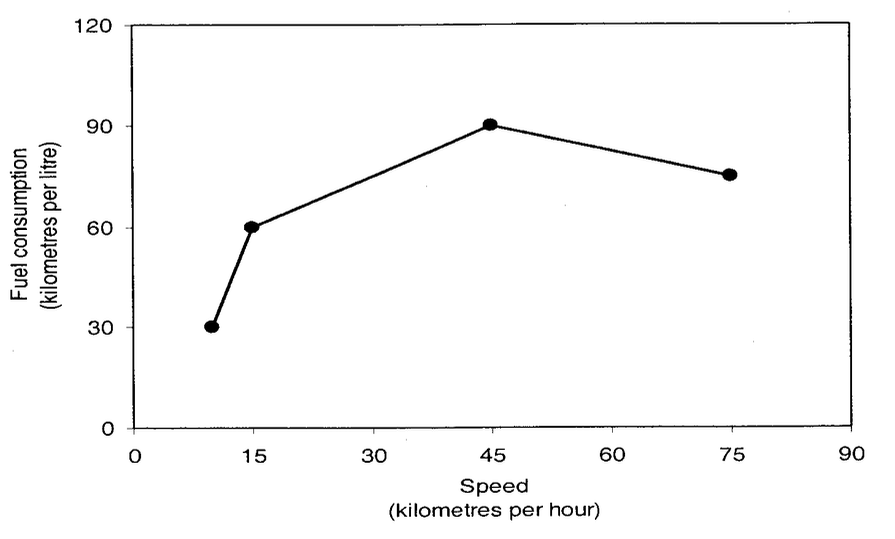
\includegraphics[width=0.7\textwidth]{project2.png}
    \caption{}
    \label{fig:project2.jpeg}
\end{figure}


\noindent
\textbf{The distances covered during four laps of the journey are listed in the table below:}

\vspace{0.5em}
\begin{center}
\begin{tabular}{|c|c|c|}
\hline
\textbf{Lap} & \textbf{Distance (kilometres)} & \textbf{Average speed (kilometres per hour)} \\
\hline
P & 15 & 15 \\
Q & 75 & 45 \\
R & 40 & 75 \\
S & 10 & 10 \\
\hline
\end{tabular}
\end{center}

From the given data, we can conclude that the fuel consumed per kilometre was \textbf{least} during the lap 

\begin{multicols}{4}
\begin{enumerate}
   \item P
   \item Q
   \item R
    \item S
\end{enumerate}
\end{multicols}


\item \textbf{The horse has played a little known but very important role in the field of medicine. Horses were injected with toxins of diseases until their blood built up immunities. Then a serum was made from their blood. Serums to fight with diphtheria and tetanus were developed this way.}

It can be inferred from the passage, that horses were
\hfill{\text{GATE MA 2011}}

\begin{enumerate}
    
    \item given immunity to diseases
    \item generally quite immune to diseases
    \item given medicines to fight toxins
    \item given diphtheria and tetanus serums
\end{enumerate}



\item  The sum of $n$ terms of the s
\hfill{\text{GATE MA 2011}}
\begin{enumerate}
    \item $(4/81) [10^{n+1} - 9n - 1]$
    \item $(4/81) [10^{n+1} - 9n - 1]$
    \item $(4/81) [10^{n+1} - 9n - 10]$
    \item $(4/81) [10^{n} - 9n - 10]$
\end{enumerate}

\item  Given that $f(y) = |y| / y$, and $q$ is any non-zero real number, the value of  \\$\left| f(q) - f(-q) \right|$ is
\hfill{\text{GATE MA 2011}}

\begin{multicols}{4}
\begin{enumerate}
   \item 0
   \item -1
   \item 1
    \item 2
\end{enumerate}
\end{multicols}

 

\begin{center}
    \textbf{END OF THE QUESTION PAPER}
\end{center}



\end{enumerate}

\end{document}
